\chapter{Implementation einer AR Anwendung für Android}
Im Rahmen des Praxisteils dieser Arbeit ist eine Applikation für Android basierte Smartphones erstellt worden. In diesem Abschnitt werden die verwendeten Tools und Frameworks, um die Augmented Reality Anwendung zu erstellen, beschrieben. Das im folgenden vorgestellte Framework ARCore, implementiert den Simultaneous Location and Mapping Ansatz und ist als einzige AR-Programmierschnittstelle Open Source (Siehe Tabelle S.29).



\section{ARCore}
ARCore, das von Google entwickelt wird und das seit März 2018 veröffentlicht wurde, ist der Nachfolger des ebenfalls von Google ins Leben gerufene Projekt Tango, welches jedoch spezielle \glqq Time-of-flight\grqq{} (TOF) Kameras benötigt, um Distanzen im Raum mithilfe des Lichtlaufzeitverfahrens zu messen. Dieser Ansatz hat sich wegen der fehlenden technischen Voraussetzungen der meisten Android Geräte nicht durchgesetzt. Da Google mit dem von Apple veröffentlichen Framework ARKit gleichziehen wollte, wurde Projekt Tango beendet und durch ARCore ersetzt. ARCore verwendet drei Schlüsselfunktionen um virtuelle Objekte in die reale Welt zu integrieren (vgl. \cite{arcore}):

\begin{itemize}
\item \textbf{Motion Tracking} ermöglicht es dem Smartphone seine Position relativ zur Umgebung zu verfolgen und zu verstehen.

\item \textbf{Environmental understanding} ermöglicht es dem Smartphone die Größe und Lage aller Arten von Oberflächen  zu erfassen, dazu zählen horizontale, vertikale oder schräge Oberflächen.

\item \textbf{Light estimation} ermöglicht die Abschätzung der aktuellen Lichtverhältnisse in der Umgebung, zur korrekten Beleuchtung und zur Erstellung von Schatten.
\end{itemize}

\subsection{Unterstütze Geräte}
Um eine gute und flüssige Erfahrung für den Endnutzer zu gewährleisten, müssen unterstützte Smartphones bestimmte Kriterien erfüllen. Dazu zählen die Qualität der verbauten Kamera, der Bewegungssensoren und der Designarchitektur. Weiterhin muss das Gerät über eine leistungsstarke CPU verfügen, die sich in das Hardware-Design integriert, um gute Leistung und effektive Echtzeitberechnung zu gewährleisten. Die Voraussetzungen um ARCore zu verwenden, werden wie folgt definiert:

\begin{itemize}
\item \textbf{Android 7.0} oder höher (Einige Modelle benötigen neuere Versionen).
\item Ein Gerät, das ursprünglich mit dem \textbf{Google Play Store} ausgeliefert wurde.
\item \textbf{Internetzugang}, um Google Play Services für AR zu installieren oder zu aktualisieren.
\end{itemize}

Aktuell werden 144 Android Smartphones unterstützt, die mit dem Google Play Store ausgeliefert werden. Weiterhin werden 29 chinesische Modelle unterstützt, bei welchen die Google Play Services manuell über die App Stores der Hersteller installiert werden müssen. Auch 20 iOS Smartphone Modelle können ARCore verwenden, dabei benötigt ARCore jedoch ARKit kompatible Geräte mit iOS 11.0 oder höher (Stand 22.08.2019, vgl. \cite{arcore_devices}).

Die aktuell unterstützten Geräte sind die Flaggschiffe der größen Smartphonehersteller seit ungefähr 2017. Google zielt mit ARCore also auf Leistungsstarke Hardware ab, um eine stabile Performance zu ermöglichen, versucht aber gleichzeitig so viele Endnutzer wie möglich zu erreichen.

\subsection{Grundlegende Konzepte}

In diesem Abschnitt werden grundlegende Schlüsselfunktionen von ARCore, wie in Kapitel 6.1 bereits eingeführt, genauer erläutert, sowie ein Einblick in die Pipeline hinter ARCore gegeben.

\textbf{Motion Tracking} wird in ARCore mit einem Prozess namens \glqq Concurrent Odometry and Mapping\grqq{} (COM) ermöglicht. Dabei werden Features im Kamerabild erkannt und zur Bestimmung der Änderung der Position des Smartphones verwendet. Diese visuellen Informationen werden mit Trägheitsmessungen der internen Messeinheiten (IMU) des Smartphones kombiniert, um die Position und Ausrichtung der Kamera relativ zur Umwelt zu bestimmen.

Google hat sich das System und die Methodik hinter \glqq Concurrent Odometry and Mapping\grqq{} patentieren lassen. Die Beschreibung des Patents und des Systems hinter COM zeigt viele Zusammenhänge des implementierten Systems in ARCore mit SLAM und photogrammetrischen Verfahren (vgl. \cite{patent}): 

\glqq \textit{An electronic device tracks its motion in an environment while building a three-dimensional visual representation of the environment that is used to correct drift in the tracked motion. A motion tracking module estimates poses of the electronic device based on feature descriptors corresponding to the visual appearance of spatial features of objects in the environment. A mapping module builds a three-dimensional visual representation of the environment based on a stored plurality of maps, and feature descriptors and estimated device poses received from the motion tracking module. The mapping module provides the three-dimensional visual representation of the environment to a localization module, which identifies correspondences between stored and observed feature descriptors. The localization module performs a loop closure by minimizing the discrepancies between matching feature descriptors to compute a localized pose. The localized pose corrects drift in the estimated pose generated by the motion tracking module.}\grqq{}


\begin{figure}[H]
	\centering
	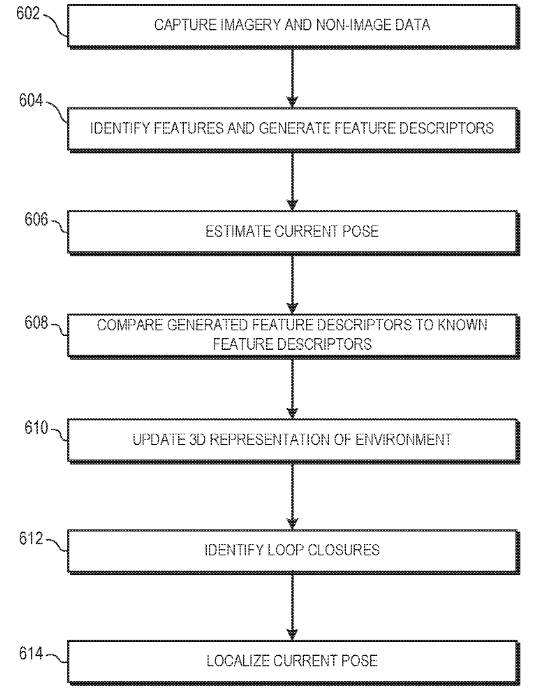
\includegraphics[scale=0.65]{com.png}
	\caption{Pipeline von COM. Bildquelle \cite{patent}}
\end{figure} 

Auch die Abbildungen über die Pipeline von COM im Patent zeigen eine hohe Übereinstimmung mit der photogrammetrischen Pipeline, sowie gegenüber SLAM (siehe Abbildung 6.1.). 

Concurrent Odometry and Mapping kann als Implementation des SLAM Verfahrens von Google interpretiert werden. Der Begriff Odometrie, der aus der Messung der realtiven Positionierung von Fahrzeugen anhand deren Eigenbewegung kommt (vgl. \cite{odometrie} S.7-9), wurde für Smartphones übernommen. Dies liegt wohl hauptsächlich in der dadurch möglichen Abgrenzung zu anderen Verfahren, für die einfachere Patentierung der Methode von Google. 


\textbf{Environmental Understanding} wird in ARCore durch die Erkennung von Clustern von Feature Punkten auf üblichen horizontalen oder vertikalen Flächen ermöglicht. Weiterhin können die Grenzen dieser Ebenen bestimmt werden. Da ARCore zur Erkennung der Ebenen Features verwendet, werden flache oder texturlose Oberflächen, wie beispielsweise eine weiße Wand möglicherweise nicht richtig erkannt. 

\textbf{Light Estimation} wird in ARCore verwendet, um Informationen über die Beleuchtung der Umgebung zu erhalten. Dazu werden Daten wie durchschnittliche Intensität der Helligkeit oder Farbtemperatur erfasst. Anhand dieser Informationen kann mit einer Helligkeitsanpassung oder Farbkorrektur das Gefühl von Realismus in der Szene verstärkt werden, indem virtuelle Objekte unter den gleichen Bedingungen wie die echte Welt beleuchtet werden. Weiterhin kann ARCore bestimmen aus welcher Richtung natürliches oder künstliches Licht kommt. Anhand dieser Informationen werden von ARCore Schatten berechnet und in der Szene gerendert.

\textbf{User Interaction} wird in ARCore mit Hilfe von \glqq Hit-Testing\grqq{} ermöglicht. Eine $(x,y)$ Koordinate auf dem Bildschirm des Smartphones wird mithilfe eines Strahls (Ray) in das Kamerabild projiziert. Alle Schnittpunkte mit Ebenen oder Merkmalspunkten des Strahls werden zusammen mit der Pose dieses Schnittpunktes zurückgegeben. Dadurch können Nutzer mit virtuellen Objekten interagieren. Es über die Touchsteuerung möglich die virtuellen Objekte zu verschieben und in ihrer Größe zu transformieren. 

\textbf{Anchors und Trackables} (Anker und trackbare Objekte) werden verwendet, da sich die Positionen von Flächen verändern kann, wenn ARCore im Lokalisierungsprozess das Verständnis für die eigene Position und das Umfeld verbessert. Um ein virtuelles Objekt zu platzieren, muss ein Anker erstellt werden, um sicherzustellen, dass ARCore die Position dieses Objekts über die Zeit verfolgt. Ebenen und Punkte sind hier eine spezielle Art von Objekt, das als \glqq Trackable\grqq{} bezeichnet wird. \\ \\ Virtuelle Ojekte können an bestimmten Trackables verankert werden, um sicherzustellen, dass die Beziehung zwischen virtuellen Objekt und dem zu verfolgenden Punkt oder der zu verfolgenden Ebene stabil bleibt, auch wenn sich das Gerät bewegt. Das heißt, dass virtuelle Objekte, die beispielsweise auf einem gewissen Punkt am Boden platziert werden, immer noch auf exakt der gleichen Position bleiben, auch wenn die Ebene, die den Boden repräsentiert, durch ARCore angepasst und verschoben wird.

\textbf{Augmented Images} ist eine Funktion, mit der Augmented Reality Anwendungen erstellt werden können, die auf bestimmte 2D-Bilder, wie beispielsweise Produktverpackungen oder Filmposter reagieren können. Diese registrierten Bilder funktionieren nach dem Prinzip von Markern. Deshalb ist es wichtig, dass genügend Merkmale im Bild vorhanden sind.\\

\begin{figure}[H]
	\centering
	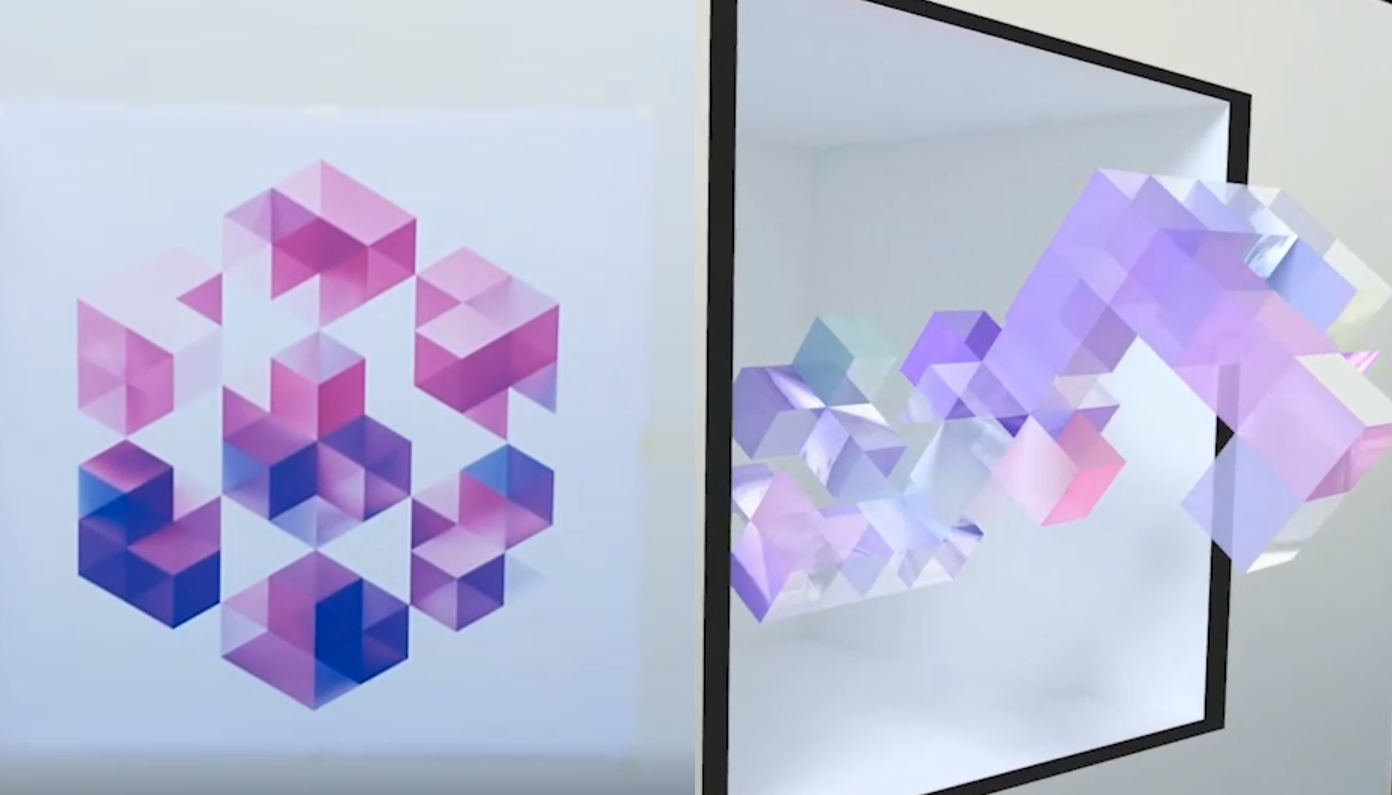
\includegraphics[scale=0.45]{augmented.png}
	\caption{Augmented Image mit ARCore, Bildquelle \cite{augmented_images}}
\end{figure} 

ARCore bietet auch eine Funktion um sich zu bewegende Bilder zu verfolgen, wie beispielsweise eine Plakatwand, auf der Seite eines fahrenden Busses. Die Bilder können offline zusammengestellt werden, um eine Bilddatenbank zu erstellen, es ist jedoch auch möglich einzelne Bilder in Echtzeit vom Gerät hinzuzufügen. Nach der Registrierung erkannt ARCore diese Bilder, sowie die Grenzen dieser und gibt eine entsprechende Pose eines virtuellen Objekts zurück. Das Bild wird von einer 2D Ansicht auf eine virtuelle 3D-Ansicht augmentiert.

Mithilfe der \textbf{ARCore Cloud Anchor API} können kollaborative AR Multiplayer Anwendungen erstellt werden. Dazu wird von einem Gerät der Anker eines virtuellen Objekts, sowie die Feature Points der näheren Umgebung, um dieses Objekt, in der Cloud gespeichert. Diese Anker können dann mit anderen Benutzern auf Android- oder iOS-Geräten in der selben Umgebung geteilt werden. Mit dieser Methode können zwei Endgeräte die gleiche virtuellen 3D-Objekte an exakt der gleichen Stelle im Raum rendern, so dass beide Benutzer das gleiche virtuelle Erlebnis teilen (vgl. \cite{fundamental_concepts}).

\subsection{Entwicklungsumgebungen}

ARCore kann mit vielen gängigen Entwicklungsumgebungen verwendet werden. Dazu zählen Android Studio, Android Native Development Kit, Unity für Android, Unity für iOS, Unreal Engine und iOS (vgl. \cite{develop}). Im Rahmen dieser Arbeit wurde Android Studio in der Version 3.4.1, sowie ARCore in der Version 1.11.0 verwendet.

\section{Sceneform}
Sceneform ist eine Framework, das von Google entwickelt wurde und welches nahtlos in ARCore integriert werden kann. Es ermöglicht das einfache Rendern von realistischen 3D-Szenen in AR- und Nicht-AR-Anwendungen, ohne bei der Programmierung auf OpenGL zurückgreifen zu müssen. Sceneform bietet folgende Features (vgl. \cite{sceneform}):

\begin{itemize}
\item Einen \glqq high-level\grqq{} \textbf{Szenengraph API}.
\item Einen realistischen \textbf{physikalischen Renderer} namens \textbf{Filament}.
\item Ein \textbf{Android Studio-Plugin} zum Importieren, Anzeigen und Erstellen von \textbf{3D-Assets}.
\end{itemize}

Sceneform benötigt Android Studio Version 3.1 oder höher und wird als Plugin installiert. Es liefert ein sogenanntes \glqq ArFragment\grqq{} welches automatisch das ARCore Session Management übernimmt, sowie die notwendigen ARCore Laufzeitprüfungen durchführt. Dazu gehört die automatische Überprüfung von kompatiblen Versionen der Google Play Services für Augmented Reality und die Überprüfung der Berechtigung für Kamera und anderer Sensoren. Sind alle Überprüfungen erfolgreich, erstellt das ArFragment eine \glqq ArSceneView\grqq{} und eine ARCore Session. Mithilfe der ArSceneView kann nun das Kamerabild gerendert werden, sowie mithilfe eines \glqq PlaneRenderers\grqq{} die erkannten Ebenen zur Platzierung von virtuellen Objekten visualisert werden.

Der ArSceneView ist eine Szene zugeordnet, welche eine baumartige Datenstruktur beinhaltet. Die Nodes dieser Datenstruktur sind die zu rendernden virtuellen Objekte. Jedes Node enthält alle Informationen, um es zu rendern und damit zu interagieren. Dazu gehören Position, Ausrichtung, Modell, Kollisionsform und Event Listener. Nodes können mit anderen Nodes Eltern-Kind-Beziehungen formen, welche sich in einer baumartigen Struktur kristallisieren. Diese Struktur wird dann als Szenengraph bezeichnet. Bei jedem Einzelbild rendert Sceneform den Szenengraph aus Sicht der Kamera, welche durch das ARCore Tracking geführt wird (vgl. \cite{sceneform_google}). 

Filament ist eine physikalisch basierte Rendering (PBR) Engine für Android, die ihren Fokus auf Echtzeit Performance bei mobilen Geräten legt. Das Hauptziel von Filament sind GPUs der Klasse OpelGL ES 3.x. Die Hauptgesichtspunkte der Engine liegen in den Bereichen Qualität, Benutzerfreundlichkeit, Vertrautheit, Flexibilität und in der Größe der bereitgestellten Renderbibliothek. Physikalisch basiertes Rendering ist ein Verfahren, das eine genauere Darstellung von Materialien und deren Wechselwirkungen mit Licht im Vergleich zu herkömmlichen Echtzeitmodellen ermöglicht. Die Trennung von Materialien und Beleuchtung im Kern der PBR Methode macht es einfacher, realistische Objekte zu erstellen, die unter allen Lichtverhältnissen präsize aussehen (vgl \cite{filament}). 

In der Implementierung der App wird Sceneform in der Version 1.11.0 verwendet.


\section{Google Places API}

Im Rahmen dieser Arbeit wird die Google Places API verwendet. Diese ermöglicht die Abfrage von Informationen mithilfe des aktuellen Standort des Smartphones. Die Places API ist ein Dienst, der Informationen über bestimmte Orte als Antwort auf eine HTTP-Anfrage zurückgibt. Places sind innerhalb der API als Einrichtungen, geografische Standorte oder berühmte Points of Interest definiert. Die Informationen die mit der API abgefragt werden können, sind etwa einfache Listen der näheren Orte, Details über die Orte in der Nähe oder Fotos der näheren Orte, bezogen aus der Datenbank von Google. Die API ermöglicht auch die  Autovervollständigung von Suchanfragen bestimmter Orte oder Querys. 

Jeder dieser Dienste wird als HTTP-Request aufgerufen und gibt entweder XML- oder JSON-Dateien als Antwort zurück. Alle Anfragen müssen das HTTPS Protkoll verwenden und benötigen einen eigenen API Schlüssel (vgl. \cite{places_api}).

Bei der Implementation der App wurde die \glqq Place Search\grqq{} Funktion der API verwendet. Ein Aufruf an die API schaut beispielsweise wie folgt aus:

\begin{lstlisting}[basicstyle=\small]
https://maps.googleapis.com/maps/api/place/nearbysearch/json?location=
 + LAT_LNG + &rankby=distance&keyword= + KEY_WORD + &key= + API_KEY;
\end{lstlisting}

Das Ergebnis dieser Anfrage erhält eine Vielzahl an Informationen, die anschließend weiter verarbeitet werden können. In dieser Implementierung wurden die Parameter \textbf{location}, \textbf{name} und \textbf{rating} verwendet, die aus der JSON Antwort der API entnommen werden.

\begin{figure}[H]
	\centering
	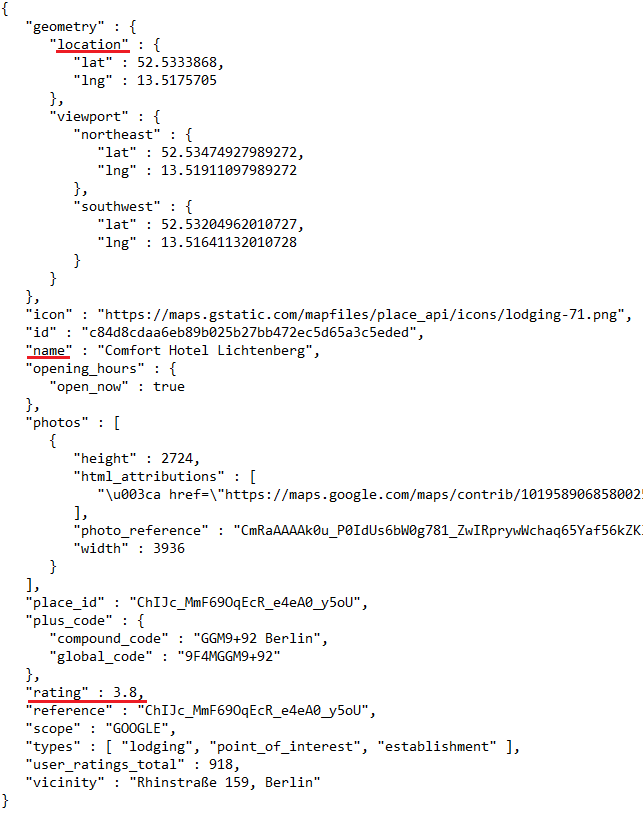
\includegraphics[scale=0.75]{location_result.png}
	\caption{Ein Ergebnis des Resultats einer Places Search mit der Google Places API}
\end{figure} 

\section{Dexter}

Dexter ist eine Open Source Android-Bibliothek der Firma Karumi, die den Prozess der Anfrage von Berechtigungen während der Laufzeit einer App vereinfacht. Seit Android Version Marshmallow (6.0), welche im Oktober 2015 veröffentlicht wurde, werden App-Berechtigungen nicht mehr bei der Installation, sondern beim Zeitpunkt der Nutzung abgefragt. Weiterhin fragt die App nur nach einer bestimmten Erlaubnis für ein Feature, wenn dieses verwendet wird (vgl. \cite{marshmallow}). Dieser neue Ansatz gibt dem Endnutzer mehr Kontrolle über die Berechtigungen seiner Anwendungen, erfordert jedoch auch die Implementation dieser Features durch den Entwickler. 

\begin{figure}[H]
	\centering
	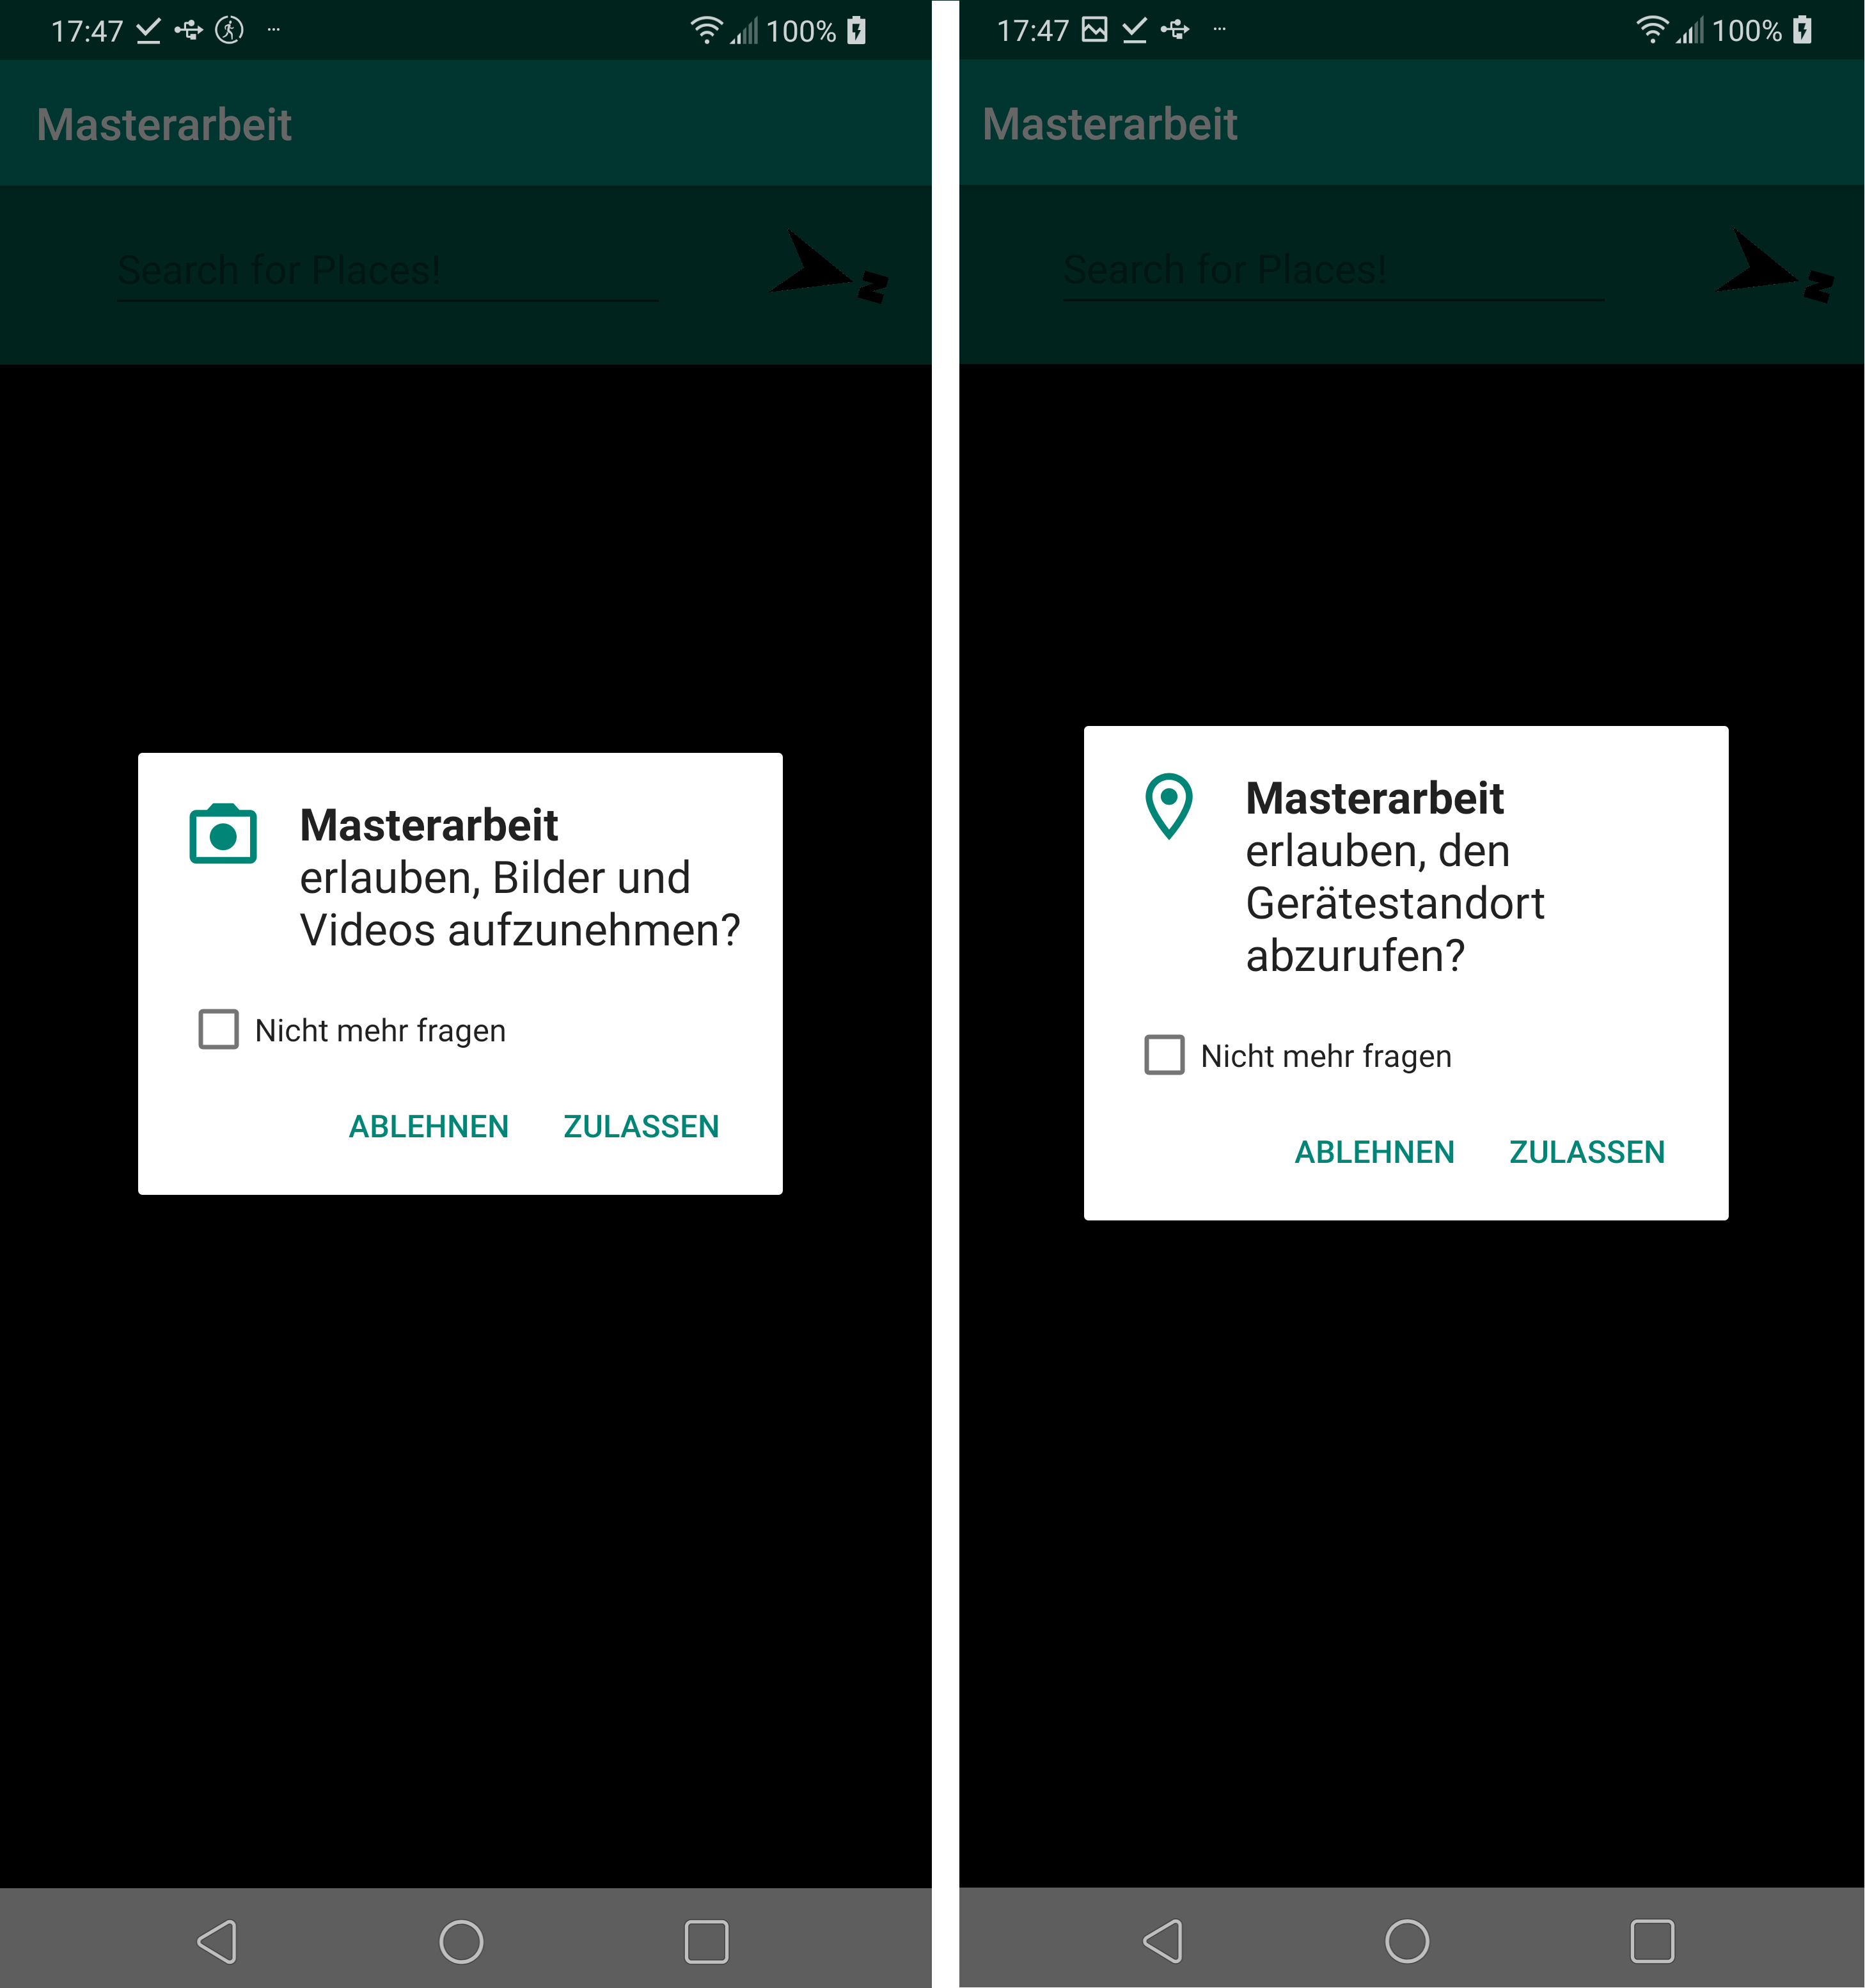
\includegraphics[scale=0.14]{request.png}
	\caption{Abfrage der Berechtigungen mit Dexter, während des Programmstarts.}
\end{figure} 

Die offizielle API zum Abfragen der Berechtigungen ist tief mit der Android \glqq Activity\grqq{} Klasse verbunden. Mit Dexter kann man die App Berechtigungen auch ohne Activities und zu einem beliebigen Zeitpunkt abfragen. Weiterhin kann die Logik überall implementiert werden (vgl. \cite{dexter}). Mit Dexter werden, beim ersten Starten der Anwendung, in der hier erstellten Applikation die Berechtigungen für Kamera und Standort abgefragt.

\section{Konzept}

Die grundlegende Idee, auf der die Anwendung aufbaut, ist es, den Nutzer nach beliebigen Informationen - in Bezug auf seinen aktuellen Standort - suchen zu lassen und die Resultate dann in der Augmented Reality anzuzeigen. So kann sich der Nutzer beispielsweise Informationen über die nächsten Hotels in der Umgebung anzeigen lassen. Die Suchanfrage wird mit der Google Places API verarbeitet. Die abgefragten Informationen werden dann von der Anwendung in Echtzeit sortiert, die Entfernungen und Himmelsrichtungen berechnet und auf zweidimensionale Infoboxen gerendert. Diese virtuellen Modelle können dann vom Benutzer platziert werden. Die Infoboxen geben dem Nutzer Auskunft über die Entfernung, die durchschnittliche Bewertung und die Himmelsrichtung der drei nächsten Points of Interest.

\section{Anwendungsbeispiel}

Nach dem Starten der App und dem Bewilligen der angeforderten Berechtigungen für Kamera und Position, wird das initiale Layout, wie in Abbildung 6.5 links zu sehen, angezeigt. Zuerst wird die aktuelle Position des Nutzers mittels GPS bestimmt. Ist die Bestimmung erfolgreich wird dies, wie in Abbildung 6.5 (1) zu sehen, in einer Benachrichtigung im unteren Bildschirmrand angezeigt. Die animierte Hand mit Smartphone, zu sehen in Abbildung 6.5 (2), ist Teil des ArFragments von ARCore und symbolisiert dem Nutzer, dass er sein Gerät in alle Richtungen drehen und bewegen soll, damit die initiale interne Positionsbestimmung der Bodenebene durchgeführt werden kann. 

Die Dauer dieser initialen Bestimmung ist abhängig von der Hardware (Kameraqualität, Rechenleistung und IMU Sensoren) und der Beleuchtungsintensität der Umgebung. Bei Tageslicht dauert die Bestimmung der initialen Pose unter einer Sekunde, bei künstlichem Licht zwischen ein und zwei Sekunden und bei spärlichen sehr dunklen Lichtverhältnissen ungefähr drei bis fünf Sekunden. Ab einem gewissen Helligkeitsgrenzwert kann die Bestimmung nicht mehr durchgeführt werden, weshalb gute Lichtverhältnisse ausschlaggebend für die optimale Funktionsweise von ARCore sind.

In der oberen Menüleiste kann der Nutzer eine Suchanfrage eingeben, siehe Abbildung 6.5 (3). Wenn die Anfrage erfolgreich ist, wird dies wie in Abbildung 6.5 (4) im unteren Bildschirmrand angezeigt. 

\begin{figure}[H]
	\centering
	\includegraphics[scale=0.8]{initial_screen.png}
	\caption{Lokalisierung (1), Posen Initialisierung (2),  Suche nach Point of Interest (3), Anzeige der Anzahl der gefundenen Ergebnisse (4).}
\end{figure} 

Weiterhin wird der Nutzer durch verschiedene Infofenster darauf hingewiesen, wenn das GPS nicht aktiviert ist oder wenn er Modelle platzieren will, die durch eine fehlende Suchanfrage noch nicht zur Verfügung stehen, siehe Abbildung 6.6. 

Nach der durchgeführten Suche, werden im Hintergrund die Entfernungen und Himmelsrichtungen der nächsten drei gefundenen Points of Interest berechnet. Diese Informationen wie Name, Entfernung, Himmelrichtung und durchschnittliche Bewertung, werden in Echtzeit in zweidimensionale Container eingefügt, die dann von ARCore in dreidimensionale Modelle gerendert werden. \\ Durch einen Tap auf die erkannte Bodenebene, die bei ARCore standardmäßig mit weißen Punkten visualisiert wird, siehe Abbildung 6.6, können die Modelle dann platziert werden.

\begin{figure}[H]
	\centering
	\includegraphics[scale=0.7]{infobox.png}
	\caption{Infoboxen für den Nutzer und Visualisierung der erkannten Bodenebene.}
\end{figure} 

Das Ergebnis der Suchanfrage wird dann, wie in Abbildung 6.7 (1) dargestellt, in das Kamerabild eingefügt. Da die von ARCore berechneten Schatten der zweidimensionalen Infoboxen nicht ansatzweise realistisch aussehen, sind diese deaktiviert worden. Die kontextsensitive Beleuchtungsintensität der Modelle funktioniert jedoch gut und ist deshalb aktiv. Die Infoboxen zeigen die Distanz zum Zielort in Metern, sowie die Himmelrichtungen $N, S, O, W$ mit den Unterteilungen $NW, SW, SE, NE$ an. 

\begin{figure}[H]
	\centering
	\hspace*{-0.5in}
	\includegraphics[scale=0.65]{result_screen.png}
	\caption{Gerendete und Platzierte virtuelle Infokarten (1), Kompass (2).}
\end{figure} 

Wie in Abbildung 6.7 (2) dargestellt, wurde ein kleiner Kompass implementiert, da die ursprünglich geplante Rotation der Infoboxen in die korrekte Himmelsrichtung, in welcher der wirkliche Ort liegt, nicht umgesetzt werden konnte (Siehe Kapitel 6.8). 


\section{Haversin-Formel und Azimut}

Zur Bestimmung des Abstands zwischen aktuellen Standort des Nutzers und dem Ziel wurde die Haversin Formel verwendet. Mithilfe der Formel kann der Großkreisabstand von zwei Punkten auf einer Kugel anhand ihrer Längen- und Breitengrade berechnet werden \cite{haversine}: 

\begin{equation}
d = 2 \pi \sin^{-1} (\sqrt{\sin²(\frac{\phi_2 - \phi_1}{2})+\cos(\phi_1)\cos(\phi_2)\sin²(\frac{\psi_2-\psi_1}{2}})
\end{equation}

Wobei $d$ die Entfernung zwischen zwei Punkten mit Längen- und Breitengrad $(\psi,\phi)$ und $r$ der Radius der Erde ist (vgl. \cite{haversine} S.299).

Die Berechnung des Azimuts, also des Kurses angegeben durch einen Winkel, der die Himmelsrichtung vom Startpunkt des Nutzers bis zum Ziel beschreibt, wird mit folgender Formel berechnet, welche auch als \glqq Vorwärts-Azimut\grqq{} bezeichnet wird \cite{bearing}:

\begin{equation}
\theta = atan2(\sin \delta\lambda \cdot\cos\phi_2, \cos \phi_1 \cdot\sin\phi_2 - \cos\phi_2 \cdot\cos\delta\lambda)
\end{equation}

Wobei $\phi_1,\lambda_1$ der Startpunkt, $\phi_2,\lambda_2$ der Endpunkt und $\delta\lambda$   die Differenz der Längengrade ist (vgl \cite{bearing}). Die ermittelte Himmelsrichtung in Grad wird dann in die acht Kategorien der Himmelsrichtung umgewandelt.

\section{Probleme}

Die ursprüngliche Idee, die virtuellen Infoboxen richtig zur Himmelsrichtung ausgerichtet in der Augmented Reality zu platzieren, ist wegen mehrerer Probleme nicht realisierbar.

\begin{itemize}

\item \textbf{Problem 1}: Die Orientierung des von ARCore benutzen globalen Koordinatensystems ist bei jeder Session verschieden. Nur die Y-Achse ist immer nach oben orientiert, was an der Erkennung der horizontalen Flächen liegt. Die globale Orientierung der X- und Z-Achse ist jedoch immer unterschiedlich (vgl. \cite{arcore_geo}).

\item \textbf{Problem 2}: Versuche das globale Koordinatensystem anhand der internen Sensoren, wie Magnetometer und Lagesensor auszurichten, hat wegen starken Ungenauigkeit dieser Sensoren zu oft zu falschen Ergebnissen geführt. Dies hat zur Folge, dass sich bei mehreren Initialisierungen des Koordinatenraums unter gleichen Startbedingungen teils sehr verschiedene Resultate und damit Drehungen des Koordinatensystems in die falsche Richtung ergeben haben. 

\item \textbf{Problem 3}: Der Magnetfeldsensor in Smartphones ist sehr anfällig für Störungen, wenn er in Gebäuden oder in der Nähe von anderen elektronischen Geräten eingesetzt wird, was durch die sehr kleine Baugröße bedingt ist. Die unter Strom gesetzte metallische Platte, welche die Lorentzkraft misst, ist so klein, dass selbst schwache Magnetfelder diese beeinflussen können.

\item \textbf{Problem 4}: Der Großteil der Benutzer von Smartphones hat noch nie das Magnetometer oder andere interne Sensoren kalibriert. Nach der Kalibrierung der internen Sensoren ist das Ergebnis um ein Vielfaches genauer, jedoch trotzdem noch störanfällig und ungenau.
\end{itemize}

Um diese Probleme zu beheben müsste eine Methode zur Kalibrierung der internen Sensoren, beim ersten Starten der Applikation, implementiert werden. \\ \\ Weiterhin müsste ein Initialisierungsverfahren die Position, Lage und Ausrichtung des Geräts ermitteln und über einen kurzen Zeitraum messen, damit anschließend mit einem Optimierungsverfahren die gemittelte initiale Orientierung bestimmt werden kann. Dann müsste das interne Koordinatensystem von ARCore anhand dieser Daten ausgerichtet werden. Dies hätte den zeitlichen Rahmen dieser Arbeit gesprengt, weshalb als Alternative die Himmelrichtung der angefragten Points of Interest mit auf den Infoboxen angezeigt wird. In der Suchleiste der Anwendung ist ein kleiner Kompass implementiert worden, der die Himmelsrichtung des Gerätes anzeigt. 

Das von Apple entwickelte Framework ARKit hat diese globale Orientierung des Koordinatensystems bereits implementiert (vgl. \cite{arkit_global}) Bei ARCore wurde dieses Feature schön seit längerer Zeit von Entwicklern erwartet, ist jedoch noch nicht offiziell erschienen. 

\section{Erkenntnisse}

Trotz der in Kapitel 6.8 genannten Probleme ist die Entwicklung der Anwendung mit ARCore, Sceneform und Android Studio sehr intuitiv und ohne weitere Probleme verlaufen. Das verwendete Smartphone, das zum Testen in dieser Arbeit verwendet wurde, ist das \textit{LG G7 ThinkQ}, welches Android 9.0, einen Snapdragon 845 SoC (System-on-a-Chip), 4GB RAM und eine 16 MP Kamera mit 2160p mit sich bringt. 

Das Tracking von ARCore ist sehr flüssig, schnell und sehr akkurat. Die Performance des Renderings der Modelle ist auch bei Experimenten mit vielen Modellen, einer großen Anzahl an Vertices, Schatten und kontextsensitiver Beleuchtung sehr stabil. ARCore und Sceneform lassen sich einfach kombinieren, das Wegfallen von OpenGL zum Rendern der Modelle, erleichtert zusätzlich den Einstieg in die Entwicklung von AR Applikationen. Das Echtzeitsystem, welches die Schatten erzeugt, funktioniert für 3D-Modelle sehr gut, für 2D-Planes nicht wirklich. Die User Interaction, um Modelle in ihrer Größe zu verändern oder im Raum zu verschieben wurde in dieser Anwendung deaktiviert, mit normalen 3D-Modellen funktioniert dies einwandfrei. Die Einstiegshürden um AR-Anwendungen zu erstellen werden in den nächsten Jahren weiter sinken, ARCore leistet dazu einen großen Entwicklungsschritt.








